\documentclass[11pt,a4paper]{article}
\usepackage[margin=2.2cm]{geometry}
\usepackage{amsmath,amssymb}
\usepackage{booktabs}
\usepackage{multirow}
\usepackage{graphicx}
\usepackage{float}
\usepackage[font=small]{caption}
\usepackage{hyperref}

\newcommand{\wt}{wt\%}

\title{\textbf{A Physics-Informed Graph Neural Network Solubility Predictor\\
for Green-Solvent Selection in PS/PET Recycling}}
\author{Your Name\\[2pt] \small Department of Chemistry --- Exploratory Project: AI in Recycling}
\date{\today}

\begin{document}
\maketitle

\begin{abstract}
Mixed polystyrene (PS) / poly(ethylene terephthalate) (PET) waste can be separated by selective
dissolution--precipitation, but finding a suitable \emph{green} solvent and operating conditions
normally requires extensive trial and error. This work presents a solubility predictor: a two-tower
graph neural network (GNN) that predicts the Flory--Huggins interaction parameter $\chi(T)=A+B/T$ as a
learned correction to a Hansen-solubility-parameter prior and converts it into saturation solubility.
It is trained on 13\,732 COSMO-RS solubilities (Zhou \emph{et al.}, 2023; 981 solvents $\times$ 8
polymers $\times$ 2 temperatures) and evaluated on structurally unseen solvents (scaffold split), on
held-out polymers, and on 41 independent experimental data points. On unseen solvents a 5-seed ensemble
reaches $R^2=0.90$ (log$_{10}$\,\wt). On experimental data the predictor separates good from
non-solvents with AUC 0.93, against 0.74 for the Hansen baseline, and its error on measured
solubilities is slightly lower than that of COSMO-RS itself. Ablations show that the physics layer and
the censored, floored output head are the components that matter. A screening stage combines the
predictions with a mass balance and a greenness filter and returns, for each solvent, a temperature
window, polymer loading, solvent-to-waste ratio, expected PS purity, dissolution time and confidence.
For a waste containing 30\,\% PS, 20 of 41 green solvents pass, led by cyclopentyl methyl ether (CPME),
diethyl carbonate and eucalyptol, with predicted PS purities of 95.7--98.5\,\%.
\end{abstract}

%=====================================================================
\section{Introduction and problem statement}
PS and PET frequently occur together in packaging waste (cups, trays, lids, labels on bottles). Because
they contaminate each other and are difficult to separate by density or sorting alone, mixed streams are
often down-cycled or landfilled. \emph{Solvent-based} recycling offers an alternative: in selective
dissolution--precipitation, exemplified by the STRAP process~\cite{strap}, a solvent dissolves one polymer
at a chosen temperature while the others remain solid. The solid fraction is filtered off and the
dissolved polymer is recovered by precipitation or evaporation, largely retaining its molecular weight.

The bottleneck is \textbf{solvent selection}. Hundreds of candidate solvents exist, solubility depends
strongly on temperature, and the solvent should be safe and sustainable (CHEM21~\cite{chem21}).
Experimental screening is slow. Hansen solubility parameters (HSP)~\cite{hansen} are the chemist's
standard shortcut but are only moderately reliable. COSMO-RS~\cite{cosmors} is more rigorous but requires
licensed software and quantum-chemical calculations for every new molecule.

\paragraph{Aim.} \emph{Given a PS/PET waste stream, rank green solvents by their predicted ability to
dissolve PS while leaving PET solid, and give for each solvent: a temperature window, the saturation
solubility, a recommended loading, the solvent-to-waste ratio, the expected PS purity and a confidence
level.}

\paragraph{Approach.} The solubility predictor learns the mapping
$(\text{polymer},\text{solvent},T)\rightarrow\chi(T)\rightarrow$ solubility. The polymers are fixed (the
problem is defined by the waste stream), and the solvent is the search space. A separate screening stage
applies selectivity, safety and mass-balance rules to the predictions.

\paragraph{Contributions.}
\begin{enumerate}
\item A physics-informed GNN that predicts the Flory--Huggins $\chi(T)=A+B/T$ as a correction to a Hansen
prior, so that temperature enters physically and the output is interpretable.
\item Training on simulated data (COSMO-RS) and \emph{external} testing on experimental data.
\item Selectivity-aware screening with deep-ensemble uncertainty that goes from molecular structure to
process numbers (solvent amount, purity).
\item An honest analysis, with baselines, ablations and leave-one-polymer-out tests, of where the
predictor generalises (new solvents) and where it does not (new polymers).
\end{enumerate}

\paragraph{Scope.} The predictor covers the 8 polymers in the training set (EVOH, PE, PP, PS, PET, PVC,
PA6, PA66), each represented by its repeat unit in the high-molecular-weight limit. PS is treated as
atactic and amorphous, which covers general-purpose PS and EPS/XPS foams. The rubber phase of HIPS,
syndiotactic PS and styrenic copolymers (ABS, SAN, SBS) are out of scope. Chain length is not a model
input.

%=====================================================================
\section{Data}
\subsection{Training data: Zhou \emph{et al.} (COSMO-RS)}
Zhou \emph{et al.}~\cite{zhou} report COSMO-RS solubilities (\wt) of 8 polymers in 1007 solvents at room
temperature (RT, taken as 298.15\,K) and at $T_h=\min(\mathrm{bp}-1,\,120)$\,\textdegree C, together with
solvent names, CAS numbers, SMILES, boiling points, HSP and chemical classes. All 1007 SMILES parse
(983 unique molecules). Cleaning steps:
\begin{itemize}
\item 1296 $T_h$ rows of solvents without a boiling point were dropped. They are copies of the RT value
at 25\,\textdegree C.
\item 748 rows without a label were dropped (solvent boils below RT).
\item 336 duplicate molecules were dropped: one solvent is kept per canonical SMILES, preferring entries
with HSP. This also removes stereoisomer duplicates.
\item Fully miscible entries (`M', 2 rows) are right-censored at 50\,\wt.
\end{itemize}
The final set has \textbf{13\,732 rows, 981 molecules}. The regression target is
$y=\log_{10}(\text{\wt}+10^{-3})$. Rows below $10^{-3}$\,\wt\ (12\,\%) are treated as left-censored.
In the cleaned data, 14 solvents are PS-selective at RT and 104 at $T_h$
(PS $\ge 10$\,\wt, PET $\le 0.5$\,\wt).

\subsection{Descriptors}
\textbf{Solvents:} $\delta_D,\delta_P,\delta_H$ and bp from Zhou (157 solvents lack bp and 29 lack HSP).
Zhou gives no densities, so molar volume comes from the McGowan volume~\cite{mcgowan}, calibrated on 17
anchor solvents as $V=1.350\,V_x-3.98$ (mean error $\approx 4$\,\%).
\textbf{Polymers:} a hand-built table of repeat-unit SMILES, $T_g$, $T_m$, crystallinity, density and
HSP from the Polymer Handbook~\cite{polyhb}, the Hansen handbook~\cite{hansen} and, for PS,
ref.~\cite{pshsp} ($\delta = 17.6/6.1/4.1$\,MPa$^{1/2}$). Descriptors are z-scored, with the solvent
scaler fitted on training solvents only.

\subsection{External experimental test set}
The external set is never used in training. It contains 16 measured solubilities from Zhou Table~3 (all
8 polymers, 13 with numerical values) and 25 good/non-solvent pairs for PS and PET from the Polymer
Handbook and the Hansen handbook. It contains no Zhou calibration points.

\subsection{Green solvent list}
57 solvents with CHEM21/GSK categories (19 recommended, 22 problematic, 10 hazardous, 6 highly
hazardous). 54 of them are in Zhou. Boiling points and HSP for $p$-cymene, Cyrene~\cite{cyrene},
$\alpha$-pinene and GVL were added from the literature. The list is used only as a screening filter.

\subsection{Splits}
Solvents are split by Bemis--Murcko scaffold~\cite{bemis} (80/10/10, seed 42), grouped by canonical
SMILES: 784 train, 98 validation, 99 test solvents (744 scaffold groups). No molecule appears in more
than one split. Acyclic solvents form singleton groups, and the benzene scaffold (162 solvents) is kept in
training. A separate leave-one-polymer-out (LOPO) protocol tests generalisation to unseen polymers.

%=====================================================================
\section{Method}
\subsection{Physics prior}
For polymer $p$ and solvent $s$:
\begin{equation}
R_a^2 = 4(\delta_{D,p}-\delta_{D,s})^2 + (\delta_{P,p}-\delta_{P,s})^2 + (\delta_{H,p}-\delta_{H,s})^2,
\qquad
B_{\mathrm{HSP}} = \frac{V_s\,R_a^2}{4R},
\end{equation}
with $V_s$ in cm$^3$\,mol$^{-1}$, $\delta$ in MPa$^{1/2}$ and $R = 8.314$\,J\,mol$^{-1}$\,K$^{-1}$. The
prior is $\chi_{\text{prior}}(T)=0.34+B_{\mathrm{HSP}}/T$, following the classical Flory--Huggins/Hansen
link~\cite{flory,hansen}. Alone, it ranks Zhou PS solubilities with Spearman $\rho=0.66$ (RT) and
$0.41$ ($T_h$).

\subsection{Network}
\begin{enumerate}
\item \textbf{Featurisation.} RDKit~\cite{rdkit} SMILES $\rightarrow$ PyTorch Geometric~\cite{pyg}
graphs with implicit hydrogens, bidirectional edges, 31 atom features and 6 bond features. Polymer
repeat units use `*' as a dummy atom type, e.g.\ PS \texttt{*CC(*)c1ccccc1} and
PET \texttt{*OCCOC(=O)c1ccc(cc1)C(=O)*}.
\item \textbf{Two GIN towers}~\cite{gin,gine} with separate weights: 4 GINEConv layers, hidden size 128,
BatchNorm, ReLU, dropout 0.1, residual connections and sum pooling. Each embedding is concatenated with
the z-scored descriptors and passed through an MLP, giving $h_p$ and $h_s$.
\item \textbf{Interaction MLP} on $[h_p,\,h_s,\,h_p\odot h_s,\,|h_p-h_s|,\,R_a^2,\,\text{mask}]$, which
outputs $\Delta A$ and $\Delta B$. The last layer is zero-initialised, so the network starts exactly at
the Hansen prior.
\item \textbf{Flory--Huggins layer}:
\begin{equation}
A = 0.34 + \Delta A,\qquad B = B_{\mathrm{HSP}}\cdot\text{mask}+\Delta B,\qquad \chi(T)=A+\frac{B}{T}.
\end{equation}
Temperature enters the network only through this layer. For solvents without HSP, $\text{mask}=0$.
\item \textbf{Solubility head}:
$r=c_0-\operatorname{softplus}(c_1)\,\chi+c_2\,x_{\text{cryst}}$ and
$\hat y=\log_{10}\!\left(10^{r}+10^{-3}\right)$. The head is initialised from a fit of the Hansen prior.
Predicted solubility decreases monotonically with $\chi$, and the floor matches the label floor.
\item \textbf{Uncertainty}: a deep ensemble~\cite{ensemble} of 5 seeds (42--46), reported as mean
$\pm\,\sigma$.
\end{enumerate}
The network has 516k parameters. One training run takes 5--8\,min on an NVIDIA RTX~2050 (4\,GB).

\subsection{Loss and training}
\begin{equation}
\mathcal{L} = \lambda_1\,\mathrm{MSE}_{\text{cens}} + \lambda_2\,\mathcal{L}_{\text{rank}} +
\lambda_3\,\mathcal{L}_{\text{phys}}.
\end{equation}
The censored MSE penalises right-censored (`M') and left-censored ($<10^{-3}$\,\wt) rows only when the
prediction lies on the wrong side, using the raw head output $r$ to avoid vanishing gradients.
$\mathcal{L}_{\text{phys}}$ is a small L2 penalty ($\lambda_3=10^{-3}$) keeping $\Delta A,\Delta B$ close
to the prior. Training uses AdamW (learning rate $10^{-3}$, weight decay $10^{-5}$, batch 256), ReduceLROnPlateau and early
stopping on validation loss (stage~1: best epoch 71 of 101). As a sanity check, the network overfits 100
rows to $R^2=1.000$. Stage~1 trains on Zhou only. Stage~2 adds a pairwise RankNet loss ($\lambda_2=0.2$)
on the PS$-$PET margins of 649 training solvents at $T_h$.

\subsection{Screening and mass balance}
For each green solvent and each $T$ from 25\,\textdegree C to $\min(\mathrm{bp}-10,\,120)$\,\textdegree C
in 5\,\textdegree C steps, the ensemble predicts $S_{\mathrm{PS}}$ and $S_{\mathrm{PET}}$. The upper limit
of 120\,\textdegree C is Zhou's $T_h$ cap: there is no training data above it. Lower and upper bounds are
mean $\mp\,\sigma$. A condition is kept if $S^{\text{lower}}_{\mathrm{PS}}\ge 10$\,\wt,
$S^{\text{upper}}_{\mathrm{PET}}\le 0.5$\,\wt, $T<\mathrm{bp}$ and the greenness category is acceptable.
For waste mass $m$ with PS mass fraction $f_{\mathrm{PS}}$ and viscosity cap $c_{\max}$:
\begin{align}
c &= \min\!\left(0.8\,S^{\text{lower}}_{\mathrm{PS}},\; c_{\max}\right), &
m_{\text{solv}} &= m f_{\mathrm{PS}}\,\frac{100-c}{c},\\
m_{\mathrm{PET}} &= \frac{S^{\text{upper}}_{\mathrm{PET}}}{100-S^{\text{upper}}_{\mathrm{PET}}}\;m_{\text{solv}}, &
\text{purity} &= \frac{m f_{\mathrm{PS}}}{m f_{\mathrm{PS}}+m_{\mathrm{PET}}},
\end{align}
where $m_{\mathrm{PET}}$ is the worst-case PET leaching. Score
$=S^{\text{lower}}_{\mathrm{PS}}-S^{\text{upper}}_{\mathrm{PET}}+w\cdot\text{greenness}$ with $w=2$.
Confidence is \emph{high} for $\sigma<0.15$, \emph{medium} for $\sigma<0.30$ and \emph{low} otherwise,
lowered one level for solvents absent from Zhou. A worked example (100\,g waste, 30\,\% PS,
$S^{\text{lower}}_{\mathrm{PS}}=38$, $S^{\text{upper}}_{\mathrm{PET}}=0.02$, $c_{\max}=10$) gives 270\,g
solvent, 0.054\,g PET and 99.82\,\% purity, and is covered by unit tests.

An optional, order-of-magnitude \textbf{dissolution time} is estimated from a diffusion model for
0.5\,mm flakes ($D_0=10^{-10}$\,m$^2$\,s$^{-1}$), driven by $(\chi^*-\chi)$. Here $\chi^*$ is the head's
$\chi$ at 10\,\wt, since the learned $\chi$ is an effective parameter (Section~\ref{sec:interp}).

%=====================================================================
\section{Baselines}
\begin{enumerate}
\item \textbf{Hansen prior}: ranking by $\chi_{\text{prior}}$, plus a 3-parameter head fitted for
regression. The relative energy difference (RED) could not be used because no interaction radius $R_0$
is available for PS.
\item \textbf{XGBoost}~\cite{xgb}: 2048-bit Morgan fingerprints (polymer encoded as a trimer), plus
descriptors, plus $T$, for 4110 features in total. HSP-derived $R_a^2$ and $\chi_{\text{prior}}$ are
deliberately excluded to keep it a non-physics baseline.
\item \textbf{Plain two-tower GIN}: identical towers and interaction MLP, predicting $\log_{10}$\,\wt\
directly from the embeddings and $1000/T$, without the Hansen prior or the $\chi$ layer.
\end{enumerate}
All baselines use the same splits and metrics.

%=====================================================================
\section{Results}
\subsection{Unseen solvents and experimental data}
\begin{table}[H]
\centering\small
\setlength{\tabcolsep}{3.2pt}
\resizebox{\linewidth}{!}{%
\begin{tabular}{lccccccccc}
\toprule
 & \multicolumn{4}{c}{Zhou test (log$_{10}$\,\wt)} & \multicolumn{2}{c}{Selectivity} & \multicolumn{3}{c}{External (experimental)}\\
\cmidrule(lr){2-5}\cmidrule(lr){6-7}\cmidrule(lr){8-10}
Model & MAE & $R^2$ & $\rho_{\mathrm{PS}}$ RT/$T_h$ & $\rho_{\mathrm{PET}}$ RT/$T_h$ & top-10 & $\rho_{\text{margin}}$ & AUC & acc. & T3 MAE\\
\midrule
Hansen prior          & 1.176 & 0.205 & 0.68/0.39 & 0.66/0.37 & 0.30 & 0.58 & 0.74 & 0.78 & 1.59\\
XGBoost               & 0.318 & 0.888 & 0.79/0.85 & 0.71/0.87 & 0.40 & 0.87 & 0.88 & 0.80 & 1.22\\
Plain GIN             & \textbf{0.236} & \textbf{0.923} & \textbf{0.91}/\textbf{0.92} & \textbf{0.83}/\textbf{0.91} & 0.50 & 0.90 & 0.89 & 0.83 & 1.21\\
Predictor, stage 1    & 0.316 & 0.894 & 0.83/0.89 & 0.73/0.89 & 0.50 & 0.92 & \textbf{0.93} & \textbf{0.85} & 1.17\\
Predictor, stage 2    & 0.327 & 0.886 & 0.84/0.88 & 0.70/0.87 & 0.50 & 0.93 & \textbf{0.93} & \textbf{0.85} & \textbf{1.12}\\
Predictor, ensemble   & 0.300 & 0.904 & 0.86/0.89 & 0.77/0.90 & 0.50 & \textbf{0.94} & 0.91 & 0.83 & 1.18\\
\bottomrule
\end{tabular}}
\caption{Comparison with the baselines. \emph{Zhou test}: 99 scaffold-split solvents never seen in
training; MAE and $R^2$ on uncensored rows; $\rho$ = Spearman. \emph{Selectivity}: PS-over-PET at $T_h$ on
the 69 test solvents with HSP (9 selective, base rate 0.13); top-10 hit rate and Spearman of predicted
vs.\ true margin. \emph{External}: 41 experimental rows; AUC good vs.\ non-solvent; accuracy of
`predicted $\ge 1$\,\wt'; MAE (log$_{10}$\,\wt) on the 13 measured Zhou Table~3 values. For reference,
COSMO-RS itself reaches MAE 1.27 and $\rho=0.78$ on these 13 values.}
\label{tab:main}
\end{table}

\textbf{Findings.}
\begin{enumerate}
\item Every learned model far exceeds the Hansen prior ($R^2$ 0.89--0.92 vs.\ 0.21).
\item The plain GIN is best at in-distribution regression. The physics layer costs
$\Delta R^2\approx 0.03$ there.
\item The solubility predictor is best where it matters for the application: AUC on experimental data
(0.93) and the PS/PET selectivity ranking ($\rho_{\text{margin}}$ 0.92--0.94; top-10 hit rate 0.50,
nearly four times the base rate).
\item On measured solubilities its error (MAE 1.12--1.18) is slightly \emph{below} that of COSMO-RS
itself (1.27), the nominal ceiling for a model trained on COSMO-RS labels.
\end{enumerate}
34 of the 41 external solvents are in the training split, so the external test measures transfer from
simulation to experiment, not generalisation to new chemistry.

\begin{figure}[H]
\centering
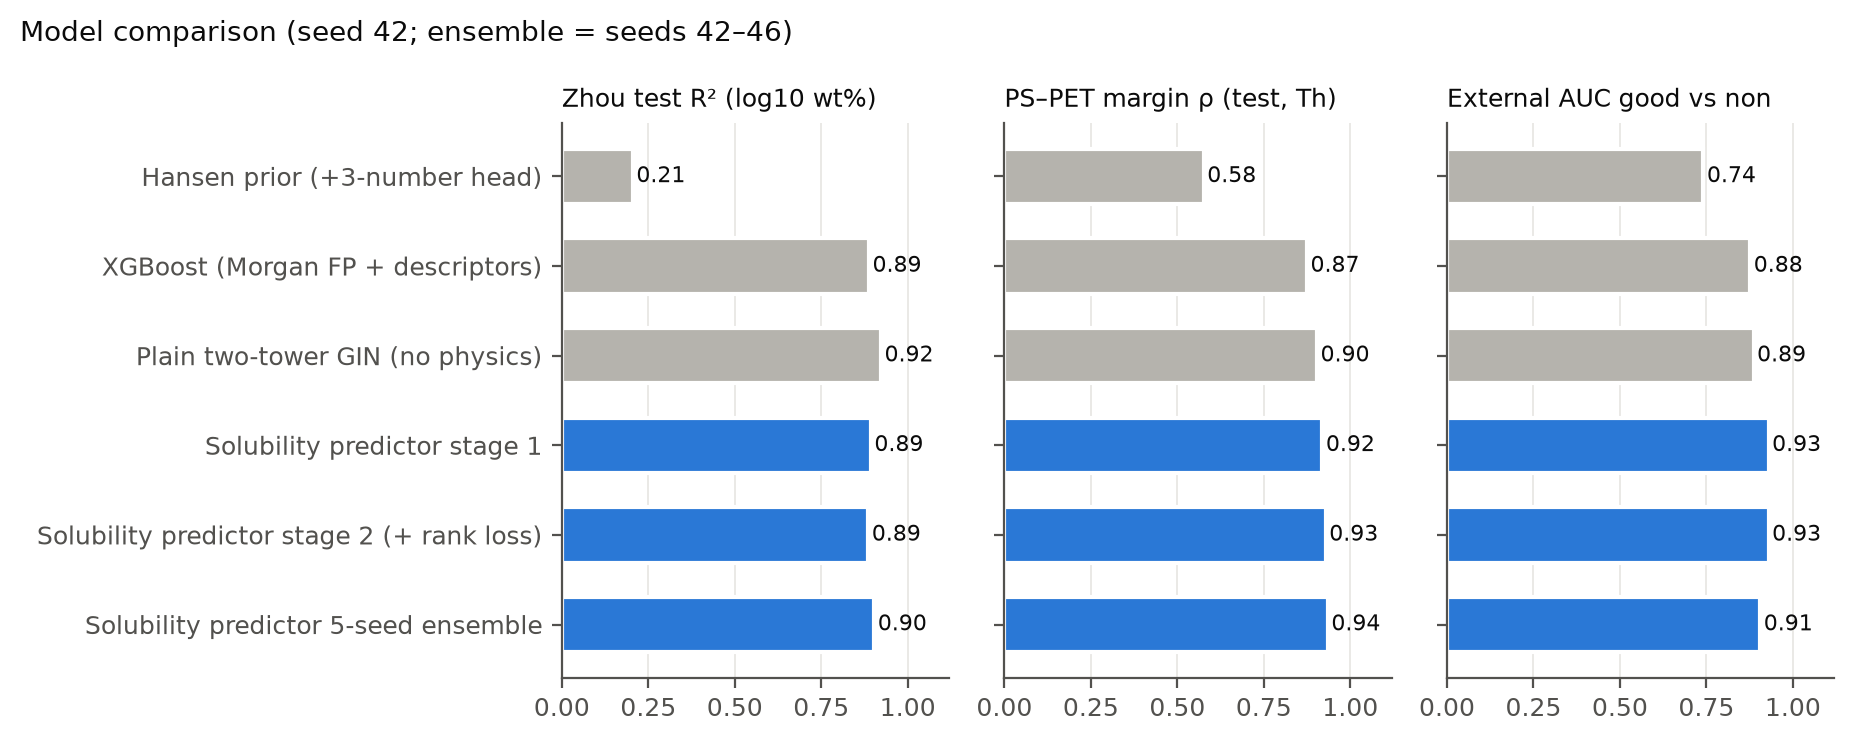
\includegraphics[width=\linewidth]{figures/fig_model_comparison.png}
\caption{Comparison with the baselines on the three test views (blue: the solubility predictor).}
\label{fig:comp}
\end{figure}

\begin{figure}[H]
\centering
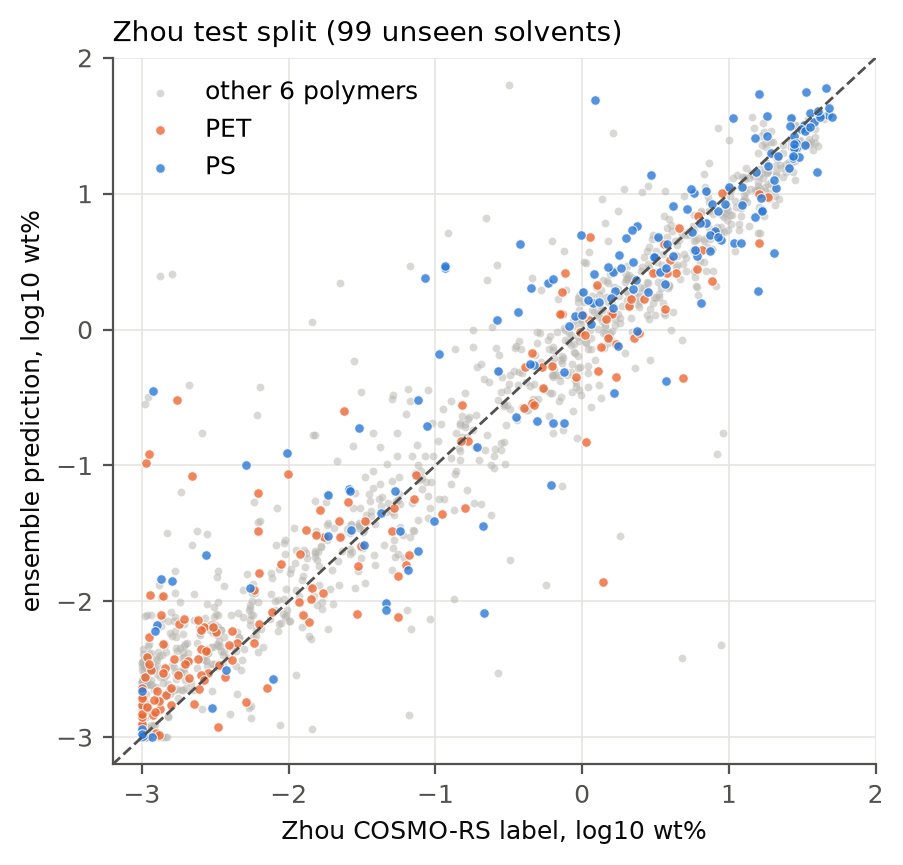
\includegraphics[width=0.6\linewidth]{figures/fig_parity_ensemble.png}
\caption{Ensemble parity plot on the Zhou test split (PS and PET highlighted).}
\end{figure}

\subsection{Ablations}
Each ablation changes one component of the stage-1 predictor and is retrained from scratch with the same
split, seed (42) and hyperparameters (Table~\ref{tab:abl}, Figure~\ref{fig:abl}). For scale, the five
ensemble members of the \emph{unchanged} model differ only in their seed and span test $R^2$ =
0.874--0.903, so single-seed differences below $\approx0.02$--$0.03$ are within noise.

\begin{table}[H]
\centering\small
\setlength{\tabcolsep}{4pt}
\resizebox{\linewidth}{!}{%
\begin{tabular}{lccccccc}
\toprule
Variant & MAE & $R^2$ & top-10 & top-20 & $\rho_{\text{margin}}$ & ext.\ AUC & T3 MAE\\
\midrule
Full predictor (stage 1)                                   & 0.316 & 0.894 & 0.50 & 0.40 & 0.92 & 0.93 & 1.17\\
$-$ physics layer (plain GIN, $1000/T$ input)              & 0.236 & 0.923 & 0.50 & 0.45 & 0.90 & 0.89 & 1.21\\
$-$ learned correction (Hansen prior + 3-number head)     & 1.176 & 0.205 & 0.30 & 0.25 & 0.58 & 0.74 & 1.59\\
$-$ floored, censored head (plain linear head)             & 0.413 & 0.863 & 0.50 & 0.40 & 0.87 & --   & --  \\
$-$ polymer descriptors                                    & 0.316 & 0.894 & 0.40 & 0.40 & 0.91 & 0.91 & 1.19\\
$-$ pair features ($h_p\odot h_s$, $|h_p-h_s|$)            & 0.276 & 0.911 & 0.40 & 0.40 & 0.88 & 0.89 & 1.19\\
Ring-closure polymer graph instead of `*' dummy atoms      & 0.280 & 0.908 & 0.40 & 0.45 & 0.89 & 0.92 & 1.16\\
$+$ PS$>$PET rank loss (stage 2)                           & 0.327 & 0.886 & 0.50 & 0.40 & 0.93 & 0.93 & 1.12\\
$+$ 5-seed ensemble                                        & 0.300 & 0.904 & 0.50 & 0.40 & 0.94 & 0.91 & 1.18\\
\bottomrule
\end{tabular}}
\caption{Ablations (seed 42). Metrics as in Table~\ref{tab:main}. `--' = not recorded for that run.
\emph{Ring closure}: the two `*' atoms are removed and their neighbours are bonded, giving a periodic
repeat-unit graph (PS: 10 $\rightarrow$ 8 nodes). \emph{Polymer descriptors}: the $T_g$, $T_m$,
crystallinity and density vector is zeroed; the crystallinity term of the head is kept.}
\label{tab:abl}
\end{table}

\begin{figure}[H]
\centering
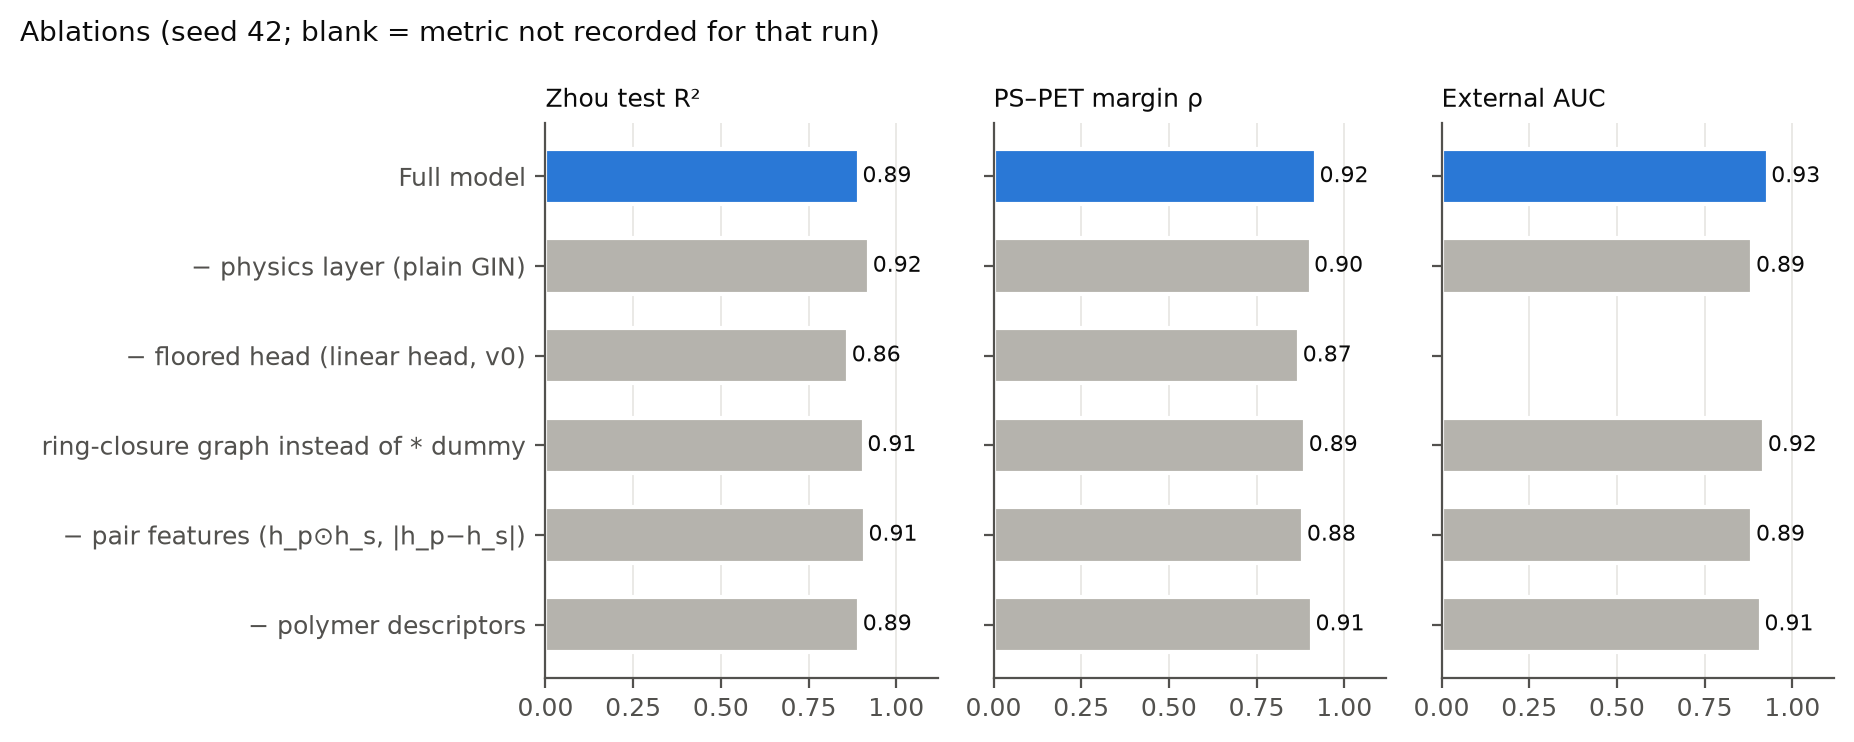
\includegraphics[width=\linewidth]{figures/fig_ablations.png}
\caption{Ablations: test $R^2$, PS--PET margin $\rho$ and external AUC.}
\label{fig:abl}
\end{figure}

\textbf{Findings.}
\begin{enumerate}
\item \textbf{Learned correction:} essential. The Hansen prior alone explains only $R^2=0.21$.
\item \textbf{Physics layer:} it trades $\approx0.03$ in-distribution $R^2$ for better experimental
transfer (AUC 0.93 vs.\ 0.89) and, decisively, for robustness on unseen polymers (LOPO,
Section~\ref{sec:lopo}).
\item \textbf{Floored, left-censored head:} $+0.03$ $R^2$ over a plain linear head, because 12\,\% of
the labels sit at the $10^{-3}$\,\wt\ floor and are no longer forced onto a straight line.
\item \textbf{Polymer descriptors:} no measurable effect. With only 8 polymers, the repeat-unit graph
already identifies each polymer uniquely, so $T_g$, $T_m$, density and crystallinity are redundant in
distribution.
\item \textbf{Pair features and dummy-atom encoding:} removing the pair features or using ring-closure
graphs gives slightly \emph{higher} test $R^2$ (0.91) but slightly \emph{lower} selectivity ranking
($\rho_{\text{margin}}$ 0.88--0.89 vs.\ 0.92) and top-10 hit rate (0.40 vs.\ 0.50). Both differences are
within single-seed noise. Neither design choice is essential; the default design is kept.
\item \textbf{Rank loss and ensembling:} small gains in selectivity ranking (0.93--0.94) within noise. The
ensemble's main benefit is the uncertainty estimate.
\end{enumerate}
In short, the components that measurably matter are the learned correction, the physics layer (for
robustness) and the censored head. The architectural details of the towers do not.

\subsection{Polymer generalisation (leave-one-polymer-out)}
\label{sec:lopo}
\begin{table}[H]
\centering\small
\begin{tabular}{lccccccc}
\toprule
Held out & $R^2$ & MAE & $\rho$ RT/$T_h$ & Plain GIN $R^2$ & Plain GIN $\rho$ RT/$T_h$ & Prior $\rho$ RT/$T_h$ & In-dist.\ $R^2$\\
\midrule
PS   & 0.01    & 1.05 & 0.64/0.78 & $-1.01$ & 0.65/0.74 & 0.66/0.41 & 0.86\\
PET  & 0.12    & 0.95 & 0.34/0.59 & $-0.94$ & 0.62/0.68 & 0.58/0.47 & 0.83\\
PE   & 0.40    & 0.93 & 0.89/0.85 & --      & --        & 0.62/0.01 & 0.93\\
PP   & $-0.29$ & 1.23 & 0.69/0.72 & --      & --        & 0.60/0.29 & 0.85\\
PVC  & 0.40    & 0.62 & 0.51/0.66 & --      & --        & 0.68/0.40 & 0.88\\
EVOH & 0.16    & 1.16 & 0.49/0.71 & --      & --        & 0.48/0.32 & 0.93\\
PA6  & 0.43    & 0.81 & 0.40/0.65 & --      & --        & 0.50/0.26 & 0.80\\
PA66 & 0.74    & 0.45 & 0.67/0.86 & --      & --        & 0.53/0.44 & 0.82\\
\bottomrule
\end{tabular}
\caption{Leave-one-polymer-out (seed 42): the held-out polymer's graph, descriptors and labels are never
seen in training; metrics on all its Zhou rows. \emph{In-dist.}: stage-1 predictor on the test split,
with the polymer seen in training. The plain GIN was run for PS and PET only.}
\label{tab:lopo}
\end{table}

The \emph{ranking} of solvents partly transfers to an unseen polymer ($\rho$ 0.34--0.89) and beats the
Hansen prior at $T_h$ for all 8 polymers. The \emph{absolute} level does not transfer ($R^2$ from
$-0.29$ to $0.74$, compared with 0.80--0.93 in distribution). With only 8 polymers, \textbf{no claim of
polymer generalisation} is made. The physics layer clearly earns its place here: for held-out PS and PET
it keeps $R^2\approx 0$--$0.1$ (MAE $\approx 1.0$), whereas the plain GIN collapses to $R^2\approx-1$
(MAE $\approx 1.6$). The plain GIN does rank PET slightly better ($\rho_{\text{RT}}$ 0.62 vs.\ 0.34).

\begin{figure}[H]
\centering
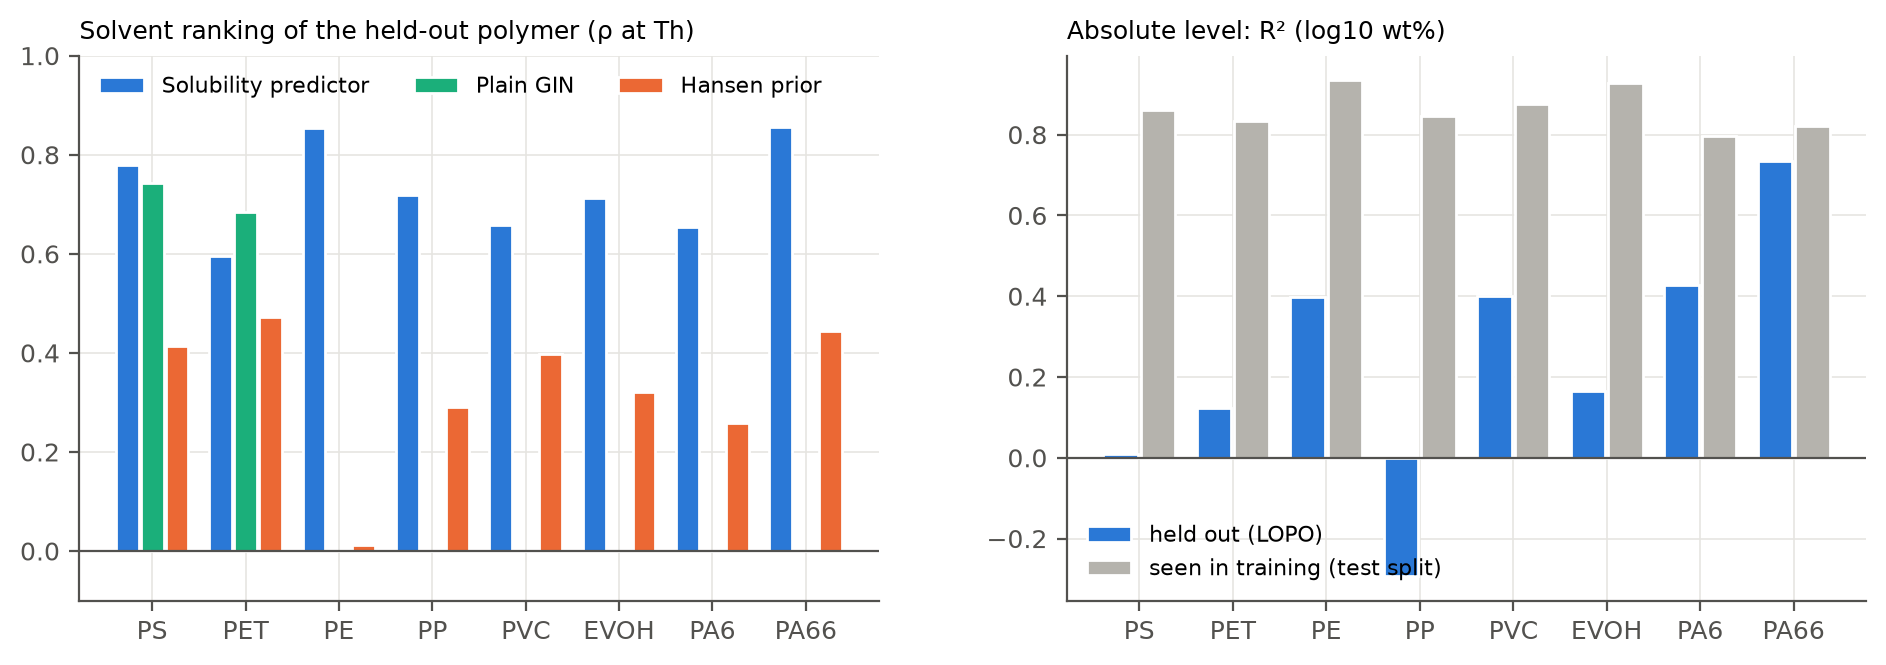
\includegraphics[width=\linewidth]{figures/fig_lopo.png}
\caption{Leave-one-polymer-out: solvent ranking at $T_h$ (left) and $R^2$ held out vs.\ seen (right).}
\end{figure}

\subsection{Uncertainty}
The ensemble $\sigma$ ranks errors usefully: Spearman$(\sigma,|e|)=0.45$. It is, however,
\textbf{overconfident}: mean $\sigma=0.13$ log units, with only 25\,\% of errors within $1\sigma$ and
47\,\% within $2\sigma$, compared with 68\,\% and 95\,\% expected for calibrated Gaussian errors
(Figure~\ref{fig:cal}). Member spread captures model disagreement but not label noise. $\sigma$ is
therefore used for ranking, for the lower and upper screening bounds, and for confidence flags, not as a
calibrated interval.

\begin{figure}[H]
\centering
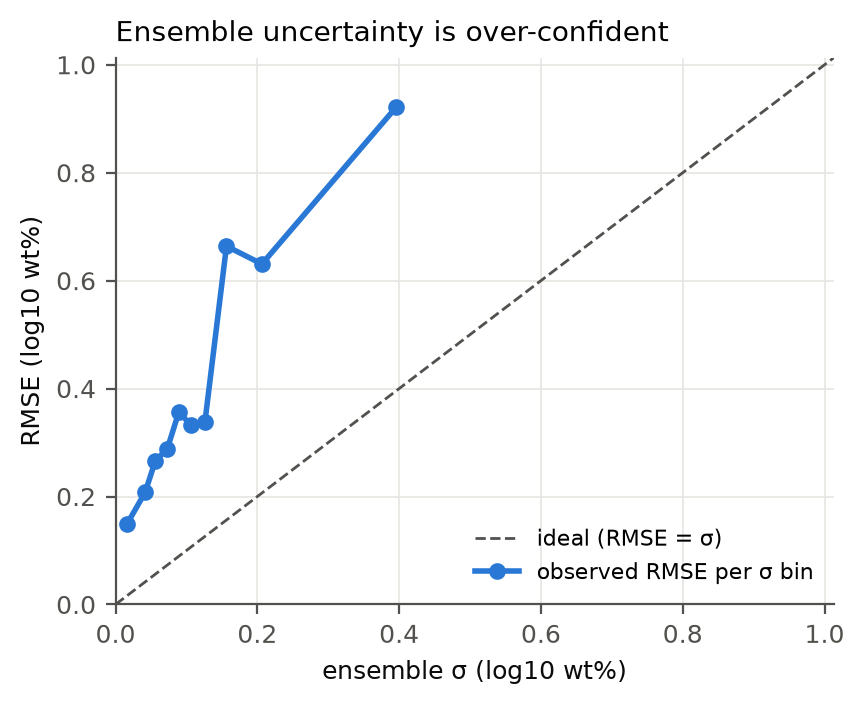
\includegraphics[width=0.5\linewidth]{figures/fig_calibration.png}
\caption{Ensemble calibration: observed RMSE per $\sigma$ bin lies above the ideal line.}
\label{fig:cal}
\end{figure}

\subsection{Interpretability: what the network learned about \texorpdfstring{$\chi$}{chi}}
\label{sec:interp}
The stage-1 test predictions include $A$, $B$, $\Delta A$, $\Delta B$ and $\chi_{\text{prior}}$ for every
row, which allows a direct comparison of the learned $\chi$ with the Hansen prior (Table~\ref{tab:chi},
Figure~\ref{fig:chi}).

\begin{table}[H]
\centering\small
\begin{tabular}{llcccc}
\toprule
Polymer & $T$ & $\rho(\chi,\chi_{\text{prior}})$ & $\rho(-\chi, y)$ & $\rho(-\chi_{\text{prior}}, y)$ & median $(A,\ B/\mathrm{K})$\\
\midrule
PS  & RT    & 0.59 & 0.83 & 0.66 & \multirow{2}{*}{$(-3.35,\ 1314)$}\\
PS  & $T_h$ & 0.28 & 0.89 & 0.33 & \\
PET & RT    & 0.62 & 0.73 & 0.61 & \multirow{2}{*}{$(-5.59,\ 2369)$}\\
PET & $T_h$ & 0.35 & 0.89 & 0.36 & \\
\bottomrule
\end{tabular}
\caption{Learned vs.\ Hansen-prior $\chi$ on the Zhou test split (stage 1).}
\label{tab:chi}
\end{table}

\begin{figure}[H]
\centering
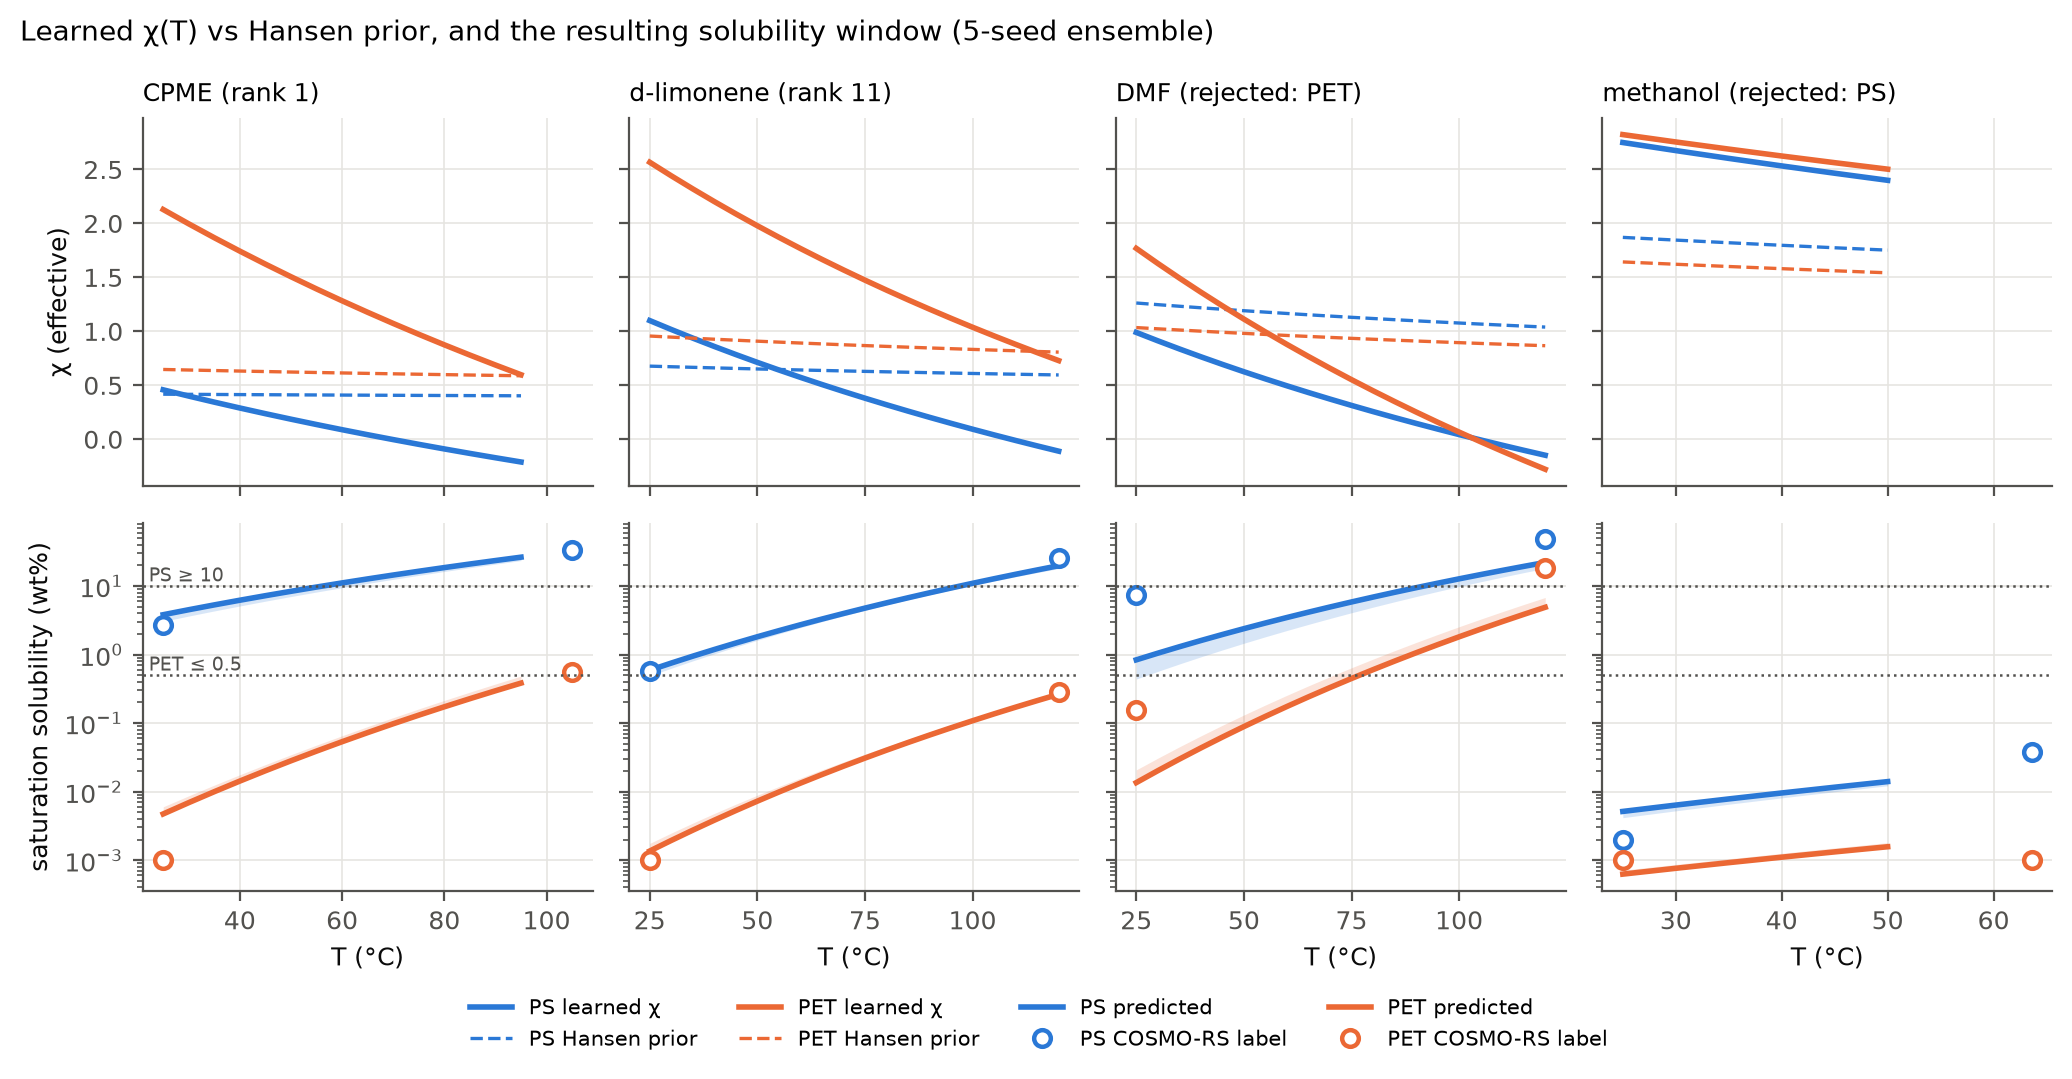
\includegraphics[width=\linewidth]{figures/fig_chi_T.png}
\caption{Top: learned $\chi(T)$ (solid) vs.\ Hansen prior (dashed) for PS and PET in two passing
solvents (CPME, d-limonene), a solvent rejected for PET leaching (DMF) and a non-solvent (methanol).
Bottom: the resulting ensemble solubility with $\pm\sigma$ band, screening thresholds (dotted) and the
COSMO-RS training labels (circles).}
\label{fig:chi}
\end{figure}

\begin{enumerate}
\item \textbf{The network keeps the prior's ordering at RT and rewrites it at high $T$.} At RT the
learned $\chi$ correlates moderately with the prior ($\rho\approx0.6$). At $T_h$ the correlation drops to
about 0.3, and the learned $\chi$ ranks solubility far better than the prior (0.89 vs.\ 0.33--0.36). The
Hansen prior's main weakness is its temperature dependence, and that is where the learned correction does
most of its work.
\item \textbf{The learned temperature dependence is much stronger than Hansen's.} For every test solvent
$B>0$, i.e.\ upper-critical-solution behaviour, with solubility rising with temperature. The median
corrections are $\Delta B\approx+1100$\,K (PS) and $+2100$\,K (PET), compensated by strongly negative $A$.
PET's larger $B$ means its solubility rises more steeply with $T$, so high temperatures erode
selectivity. In DMF (Figure~\ref{fig:chi}) the learned $\chi_{\mathrm{PET}}$ even drops below
$\chi_{\mathrm{PS}}$ above $\approx100$\,\textdegree C. This is why the screening windows have upper
bounds set by PET leaching, not only by the boiling point. Because only two temperatures per pair are
available, $A$ and $B$ are individually poorly identified (they compensate each other), so only
$\chi(T)$ over 25--120\,\textdegree C should be interpreted.
\item \textbf{The learned $\chi$ is an effective parameter.} Its absolute values do not match
Flory--Huggins theory: the head maps $\chi\approx0.1$, not 0.5, to 10\,\wt. Values below zero occur for
good solvents at high $T$, e.g.\ $\chi_{\mathrm{PS}}$ in CPME falls from 0.46 at 25\,\textdegree C to
$-0.21$ at 95\,\textdegree C, while $\chi_{\mathrm{PET}}$ falls from 2.13 to 0.60. Learned $\chi$ values
should not be compared directly with literature $\chi$.
\item \textbf{Functional-group trends are chemically sensible} (median learned $\chi$ per Zhou solvent
class, test split, classes with $\ge3$ members):
  \begin{itemize}
  \item PS at RT, best to worst: ethers (0.50) $<$ ketones (0.70) $\approx$ esters (0.71) $\approx$
  alkenes/terpenes (0.73) $<$ alkyl halides (0.99) $<$ alkanes (1.13) $\ll$ nitriles (1.91) $\approx$
  amines (1.93) $<$ alcohols (2.10) $<$ amides (2.71). This matches the classical picture of PS: soluble
  in moderately polar, non-H-bonding solvents with aromatic or ether character, insoluble in alcohols and
  strongly polar or H-bonding solvents.
  \item PET at $T_h$, best to worst: ketones (0.12) $<$ nitriles (0.24) $<$ esters (0.33) $<$ alcohols
  (0.51) $<$ ethers (0.77) $\ll$ alkanes (1.69) $<$ alkenes (2.10) $<$ alkyl halides (2.54). Polar
  aprotic carbonyl and nitrile solvents attack PET at high $T$, while hydrocarbons do not.
  \end{itemize}
  The selectivity window therefore lies in \emph{ethers and terpene-type hydrocarbons} (good for PS, poor
  for PET), with esters and ketones usable only at moderate temperatures. This is exactly the composition
  of the screening shortlist.
\end{enumerate}

\subsection{Screening: PS from PET}
Settings: 100\,g waste, 30\,\% PS, greenness category $\ge 2$, $c_{\max}=10$\,\wt.
\textbf{20 of 41} green solvents pass (Table~\ref{tab:screen}, Figure~\ref{fig:screen}). 19 of them
operate at the viscosity cap (2.7\,g solvent per g waste). Dimethyl carbonate is limited by solubility
instead (loading 8.4\,\wt, 3.3\,g/g).

\begin{table}[H]
\centering\small
\setlength{\tabcolsep}{4pt}
\resizebox{\linewidth}{!}{%
\begin{tabular}{rlccccccl}
\toprule
\# & Solvent & $T$ window (\textdegree C) & $S_{\mathrm{PS}}$ (\wt) & $S^{\text{up}}_{\mathrm{PET}}$ (\wt) & Purity (\%) & $t_{\text{diss}}$ (min) & Conf. & CHEM21\\
\midrule
1  & Cyclopentyl methyl ether     & 65--95   & 26.4 & 0.49 & 95.8 & 16 & high   & problematic\\
2  & Diethyl carbonate            & 70--100  & 23.8 & 0.50 & 95.7 & 17 & high   & problematic\\
3  & Eucalyptol (1,8-cineole)$^b$ & 95--120  & 25.9 & 0.30 & 97.4 & 16 & high   & problematic\\
4  & Butanone                     & 30--60   & 21.6 & 0.49 & 95.8 & 20 & high   & recommended\\
5  & Tetrahydrofuran              & 25--55   & 22.2 & 0.32 & 97.2 & 19 & high   & problematic\\
6  & $n$-Butyl acetate            & 65--90   & 19.5 & 0.40 & 96.5 & 23 & high   & recommended\\
7  & Methyl isobutyl ketone       & 65--85   & 19.1 & 0.40 & 96.5 & 23 & high   & recommended\\
8  & Ethyl acetate                & 45--65   & 18.6 & 0.26 & 97.7 & 25 & high   & recommended\\
9  & Toluene                      & 60--85   & 20.7 & 0.43 & 96.3 & 21 & high   & problematic\\
10 & 2-MeTHF$^b$                  & 40--65   & 19.7 & 0.16 & 98.5 & 22 & high   & problematic\\
11 & d-Limonene$^b$               & 100--120 & 19.8 & 0.29 & 97.5 & 22 & high   & problematic\\
12 & $\alpha$-Pinene$^{a,b}$      & 100--115 & 20.0 & 0.47 & 95.9 & 22 & medium & problematic\\
13 & Acetone                      & 25--45   & 16.9 & 0.36 & 96.9 & 29 & high   & recommended\\
14 & Anisole                      & 75--85   & 16.5 & 0.48 & 95.8 & 30 & high   & recommended\\
15 & Cyclohexanone                & 50--70   & 17.4 & 0.37 & 96.8 & 27 & high   & problematic\\
16 & $p$-Xylene                   & 80--95   & 19.3 & 0.45 & 96.1 & 23 & high   & problematic\\
17 & $p$-Cymene$^{a,b}$           & 60--75   & 18.1 & 0.48 & 95.8 & 25 & medium & problematic\\
18 & Isopropyl acetate            & 70--75   & 13.8 & 0.25 & 97.8 & 48 & high   & recommended\\
19 & Ethyl lactate$^b$            & 90--100  & 15.5 & 0.47 & 95.9 & 35 & high   & problematic\\
20 & Dimethyl carbonate           & 80       & 12.8 & 0.26 & 97.2 & 64 & high   & recommended\\
\bottomrule
\end{tabular}}
\caption{Passing solvents for 100\,g waste, 30\,\% PS. $S_{\mathrm{PS}}$ = ensemble mean; purity and
dissolution time at the operating temperature (upper end of the window). $^a$Not in Zhou: prediction
only. $^b$Bio-based.}
\label{tab:screen}
\end{table}

\begin{figure}[H]
\centering
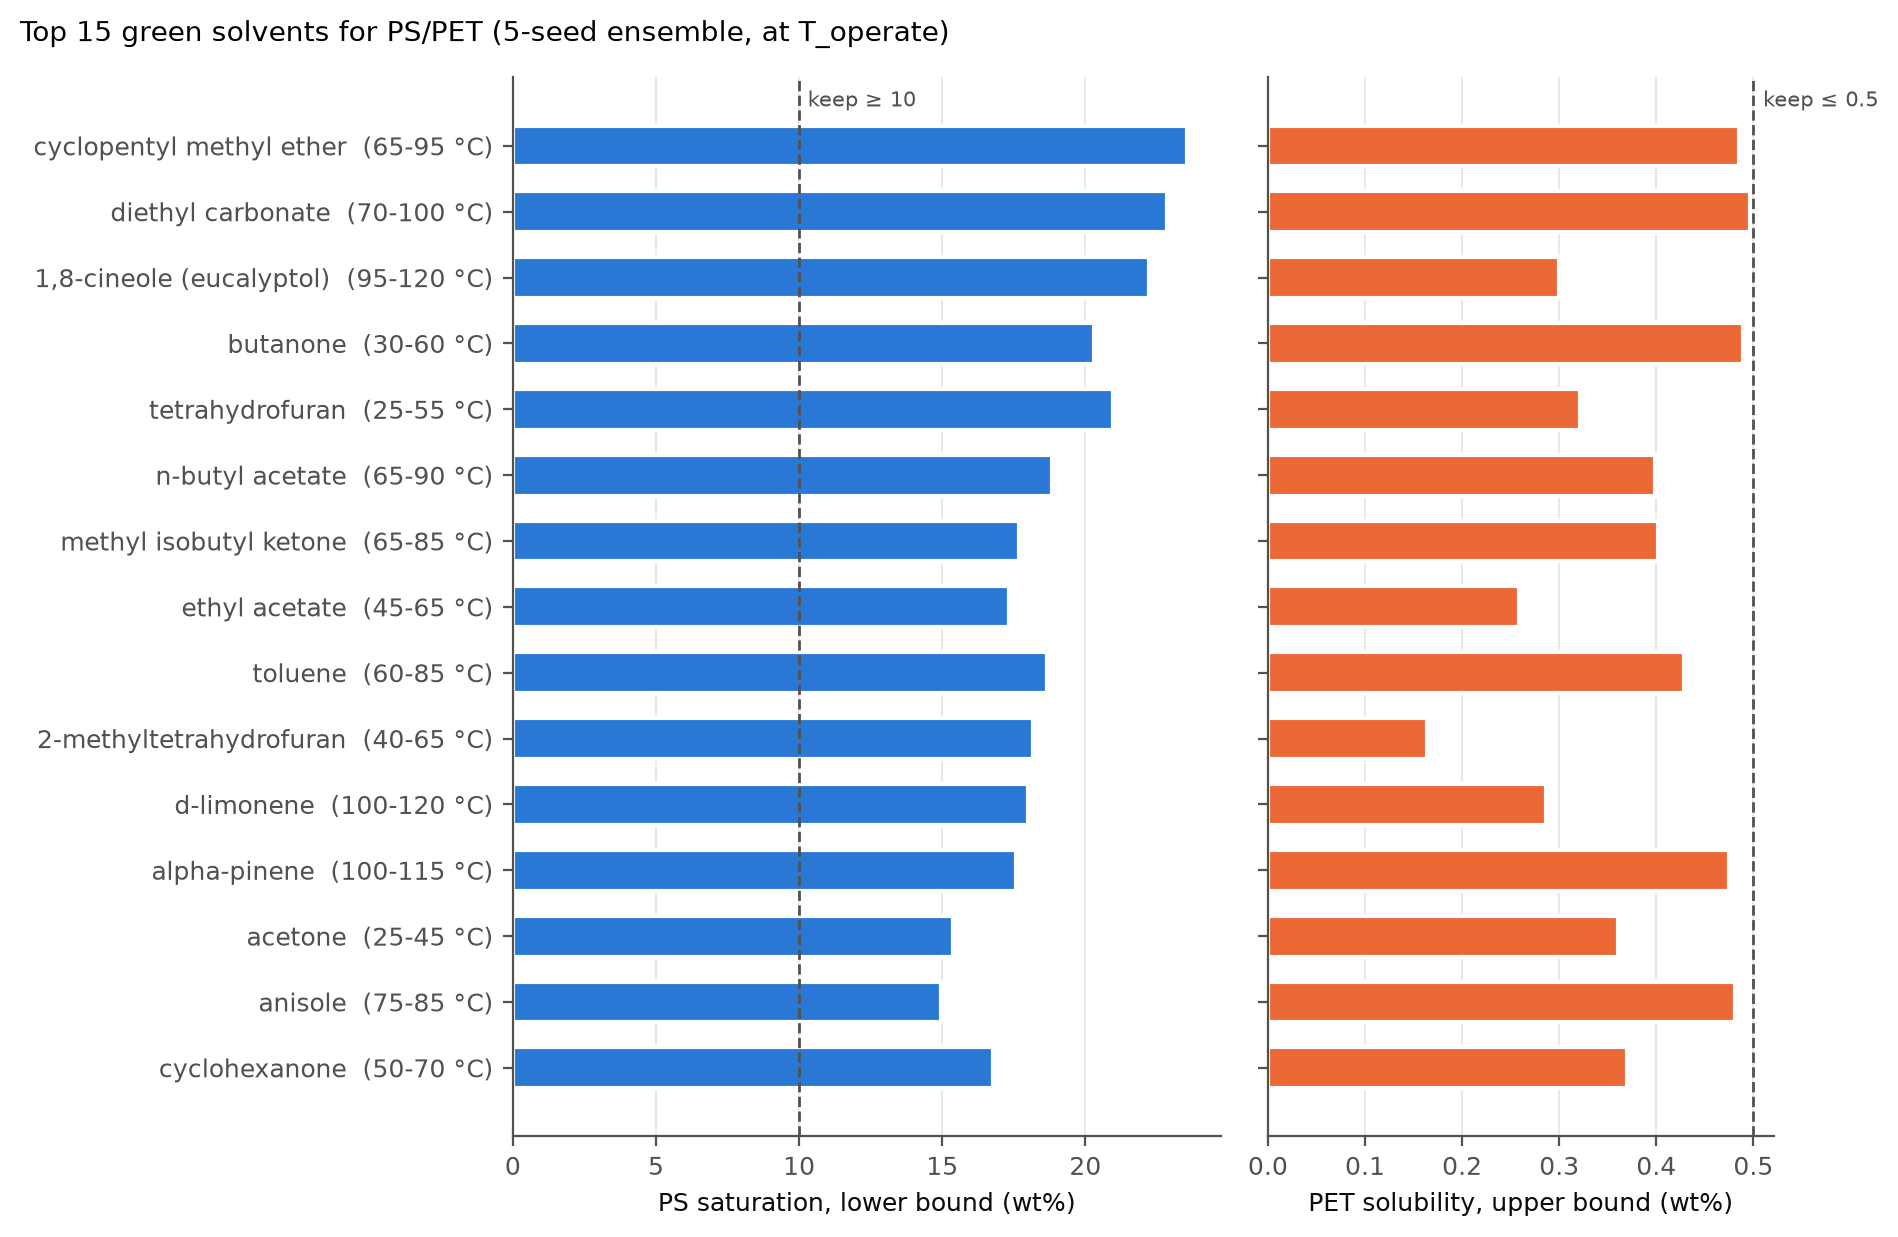
\includegraphics[width=0.85\linewidth]{figures/fig_screening_top.png}
\caption{Top 15 green solvents: conservative PS saturation (left) and worst-case PET solubility (right)
at the operating temperature, with the screening thresholds.}
\label{fig:screen}
\end{figure}

\textbf{Sanity checks.}
\begin{itemize}
\item Known PS solvents (toluene, THF, limonene) pass.
\item DMF, screened with the greenness filter disabled, is rejected at every temperature
($S^{\text{upper}}_{\mathrm{PET}}$ = 1.1--6.8\,\wt\ at 85--120\,\textdegree C), consistent with its known
ability to attack PET.
\item Alcohols, water, alkanes and glycols are rejected for low PS solubility.
\item GVL and DMSO each meet the PS and the PET threshold, but never at the same temperature.
\item Cyrene is rejected ($S^{\text{lower}}_{\mathrm{PS}}=3.9$\,\wt, prediction only).
\end{itemize}
The top-ranked solvents are CHEM21 `problematic', not `recommended'. Butanone is the best-ranked
`recommended' solvent, and 2-MeTHF and d-limonene are the strongest bio-based options. The upper end of
each window is typically set by PET leaching, which grows faster with temperature than PS solubility
(Section~\ref{sec:interp}).

%=====================================================================
\section{Discussion}
\paragraph{What the predictor is for.} It is a \emph{solvent recommender for known polymers}. The
polymers define the problem (the waste stream), and the solvents are the search space in which the
predictor has been shown to generalise (scaffold split, $R^2=0.90$).

\paragraph{Value beyond the COSMO-RS table.} For the 54 green solvents already in Zhou, a rule applied
directly to the COSMO-RS table would give a broadly similar shortlist. The predictor adds:
\begin{itemize}
\item continuous temperature windows instead of two temperatures;
\item uncertainty;
\item a small but consistent correction towards experiment (external MAE 1.17 vs.\ 1.27 for COSMO-RS);
\item and, above all, predictions for solvents without any COSMO-RS or experimental data (e.g.\
$p$-cymene, $\alpha$-pinene, Cyrene), in milliseconds from a SMILES string, without licensed software.
\end{itemize}
Screening larger libraries of emerging bio-based solvents is therefore the natural use case.

\paragraph{The physics vs.\ accuracy trade-off.} The physics layer does not maximise in-distribution
$R^2$; an unconstrained GIN does better on Zhou's test split. The physics layer instead improves
robustness where data is thin (held-out polymers, experimental data). It also enforces a monotone,
temperature-consistent $\chi(T)$ whose learned behaviour can be inspected and checked against chemical
intuition (Section~\ref{sec:interp}). The ablations confirm that this layer, not the details of the GNN
architecture, is what distinguishes the predictor from a generic GNN.

\paragraph{Chain length and composition.} Chain length is not a learned input because the training labels
contain no molecular-weight information. For commercial grades ($N\sim10^2$--$10^3$) the critical
$\chi_c=\tfrac12(1+N^{-1/2})^2$ barely changes. Molecular weight matters mainly through solution
viscosity (via $c_{\max}$) and dissolution kinetics, and could be included through physics in the
screening stage. Waste composition affects only the mass balance; the current score ranks by solubility
margin, so the shortlist does not depend on the PS fraction.

%=====================================================================
\section{Limitations}
\begin{itemize}
\item Training labels are simulated (COSMO-RS), with known misses such as PET in DMF. Experimental
agreement is bounded by COSMO-RS accuracy. The predictions have not been validated in the laboratory.
\item There are only two temperatures per pair (one for the 157 solvents without bp), so $A$ and $B$ are
poorly identified individually, and there is no training data above 120\,\textdegree C.
\item With only 8 polymers, there is no polymer generalisation (LOPO).
\item Ablations use a single seed; differences below $\approx0.02$--$0.03$ in $R^2$ are within seed
noise. The optional $\sigma$-profile feature ablation was not performed, because it needs COSMO
$\sigma$-profiles for all 981 solvents, which are not available without quantum-chemical calculations.
\item The predictor assumes the high-molecular-weight limit. Chain length, its distribution, and
degradation in recycled material are not modelled.
\item It covers atactic PS only. The HIPS rubber phase, sPS and copolymers are excluded. Real-waste
crystallinity variance (especially of PET) and additives (pigments, fillers, flame retardants) are not
modelled.
\item The ensemble $\sigma$ is overconfident.
\item The external test reuses Zhou solvents, so it tests transfer from simulation to experiment, not new
chemistry. Solvents absent from Zhou (Cyrene, $p$-cymene, $\alpha$-pinene, GVL above 25\,\textdegree C)
rely on extrapolation.
\item Hand-built polymer properties, handbook solvent pairs and CHEM21 categories are typical literature
values that have not been individually re-verified against the primary sources. The EVOH HSP is an
estimate. Eucalyptol and $\alpha$-pinene are categorised by analogy (not in CHEM21).
\item $V_s$ from the McGowan volume overestimates very large molecules (e.g.\ triolein $\approx+14$\,\%).
RT is taken as 298.15\,K.
\end{itemize}

%=====================================================================
\section{Conclusion and future work}
The solubility predictor presented here estimates the Flory--Huggins $\chi(T)$ of polymer--solvent pairs
as a learned correction to a Hansen prior and turns it into actionable dissolution conditions for PS/PET
separation. It generalises to unseen solvents ($R^2=0.90$), transfers to experimental data better than
the Hansen and data-driven baselines (AUC 0.93), and yields a ranked green-solvent shortlist led by CPME,
diethyl carbonate and eucalyptol, with butanone, 2-MeTHF and d-limonene as recommended or bio-based
alternatives. Ablations show that its advantages come from the physics layer and the censored output
head rather than from architectural details.

\textbf{Future work:}
\begin{itemize}
\item experimental testing of the top candidates on real PS/PET waste;
\item screening of large libraries of bio-based solvents outside Zhou;
\item solvent mixtures;
\item more polymers and temperatures (needed for genuine polymer generalisation);
\item molecular-weight effects through Flory--Huggins theory and viscosity in the screening stage;
\item a composition- and cost-aware score;
\item multi-seed ablations and better-calibrated uncertainty;
\item active learning with experimental data.
\end{itemize}

%=====================================================================
\begin{thebibliography}{99}
\bibitem{zhou} Zhou \emph{et al.}, \emph{Green Chem.}, 2023, \textbf{25}, 4402--4414, DOI: 10.1039/D3GC00404J.
\bibitem{strap} T.~W.~Walker \emph{et al.}, Recycling of multilayer plastic packaging materials by
solvent-targeted recovery and precipitation, \emph{Sci.\ Adv.}, 2020, \textbf{6}, eaba7599.
\bibitem{cosmors} A.~Klamt, Conductor-like screening model for real solvents, \emph{J.\ Phys.\ Chem.},
1995, \textbf{99}, 2224--2235.
\bibitem{hansen} C.~M.~Hansen, \emph{Hansen Solubility Parameters: A User's Handbook}, 2nd edn., CRC
Press, 2007.
\bibitem{flory} P.~J.~Flory, \emph{Principles of Polymer Chemistry}, Cornell University Press, 1953.
\bibitem{polyhb} J.~Brandrup, E.~H.~Immergut and E.~A.~Grulke (eds.), \emph{Polymer Handbook}, 4th
edn., Wiley, 1999.
\bibitem{pshsp} PS Hansen parameters: \emph{Materials}, 2018, \textbf{11}, 1529.
\bibitem{chem21} D.~Prat \emph{et al.}, CHEM21 selection guide of classical- and less
classical-solvents, \emph{Green Chem.}, 2016, \textbf{18}, 288--296.
\bibitem{cyrene} J.~Sherwood \emph{et al.}, Dihydrolevoglucosenone (Cyrene) as a bio-based alternative
for dipolar aprotic solvents, \emph{Chem.\ Commun.}, 2014, \textbf{50}, 9650--9652.
\bibitem{mcgowan} M.~H.~Abraham and J.~C.~McGowan, The use of characteristic volumes to measure cavity
terms in reversed phase liquid chromatography, \emph{Chromatographia}, 1987, \textbf{23}, 243--246.
\bibitem{bemis} G.~W.~Bemis and M.~A.~Murcko, The properties of known drugs. 1. Molecular frameworks,
\emph{J.\ Med.\ Chem.}, 1996, \textbf{39}, 2887--2893.
\bibitem{rdkit} RDKit: Open-source cheminformatics, \url{https://www.rdkit.org}.
\bibitem{pyg} M.~Fey and J.~E.~Lenssen, Fast graph representation learning with PyTorch Geometric,
ICLR Workshop on Representation Learning on Graphs and Manifolds, 2019.
\bibitem{gin} K.~Xu, W.~Hu, J.~Leskovec and S.~Jegelka, How powerful are graph neural networks?,
ICLR, 2019.
\bibitem{gine} W.~Hu \emph{et al.}, Strategies for pre-training graph neural networks, ICLR, 2020.
\bibitem{ensemble} B.~Lakshminarayanan, A.~Pritzel and C.~Blundell, Simple and scalable predictive
uncertainty estimation using deep ensembles, NeurIPS, 2017.
\bibitem{xgb} T.~Chen and C.~Guestrin, XGBoost: A scalable tree boosting system, KDD, 2016.
\end{thebibliography}

\end{document}
